% Options for packages loaded elsewhere
\PassOptionsToPackage{unicode}{hyperref}
\PassOptionsToPackage{hyphens}{url}
%
\documentclass[
]{article}
\usepackage{lmodern}
\usepackage{amsmath}
\usepackage{ifxetex,ifluatex}
\ifnum 0\ifxetex 1\fi\ifluatex 1\fi=0 % if pdftex
  \usepackage[T1]{fontenc}
  \usepackage[utf8]{inputenc}
  \usepackage{textcomp} % provide euro and other symbols
  \usepackage{amssymb}
\else % if luatex or xetex
  \usepackage{unicode-math}
  \defaultfontfeatures{Scale=MatchLowercase}
  \defaultfontfeatures[\rmfamily]{Ligatures=TeX,Scale=1}
\fi
% Use upquote if available, for straight quotes in verbatim environments
\IfFileExists{upquote.sty}{\usepackage{upquote}}{}
\IfFileExists{microtype.sty}{% use microtype if available
  \usepackage[]{microtype}
  \UseMicrotypeSet[protrusion]{basicmath} % disable protrusion for tt fonts
}{}
\makeatletter
\@ifundefined{KOMAClassName}{% if non-KOMA class
  \IfFileExists{parskip.sty}{%
    \usepackage{parskip}
  }{% else
    \setlength{\parindent}{0pt}
    \setlength{\parskip}{6pt plus 2pt minus 1pt}}
}{% if KOMA class
  \KOMAoptions{parskip=half}}
\makeatother
\usepackage{xcolor}
\IfFileExists{xurl.sty}{\usepackage{xurl}}{} % add URL line breaks if available
\IfFileExists{bookmark.sty}{\usepackage{bookmark}}{\usepackage{hyperref}}
\hypersetup{
  pdftitle={ADF\&G Biometrics Best Practices--DRAFT},
  pdfauthor={Ben Williams and others},
  hidelinks,
  pdfcreator={LaTeX via pandoc}}
\urlstyle{same} % disable monospaced font for URLs
\usepackage[margin=1in]{geometry}
\usepackage{color}
\usepackage{fancyvrb}
\newcommand{\VerbBar}{|}
\newcommand{\VERB}{\Verb[commandchars=\\\{\}]}
\DefineVerbatimEnvironment{Highlighting}{Verbatim}{commandchars=\\\{\}}
% Add ',fontsize=\small' for more characters per line
\usepackage{framed}
\definecolor{shadecolor}{RGB}{248,248,248}
\newenvironment{Shaded}{\begin{snugshade}}{\end{snugshade}}
\newcommand{\AlertTok}[1]{\textcolor[rgb]{0.94,0.16,0.16}{#1}}
\newcommand{\AnnotationTok}[1]{\textcolor[rgb]{0.56,0.35,0.01}{\textbf{\textit{#1}}}}
\newcommand{\AttributeTok}[1]{\textcolor[rgb]{0.77,0.63,0.00}{#1}}
\newcommand{\BaseNTok}[1]{\textcolor[rgb]{0.00,0.00,0.81}{#1}}
\newcommand{\BuiltInTok}[1]{#1}
\newcommand{\CharTok}[1]{\textcolor[rgb]{0.31,0.60,0.02}{#1}}
\newcommand{\CommentTok}[1]{\textcolor[rgb]{0.56,0.35,0.01}{\textit{#1}}}
\newcommand{\CommentVarTok}[1]{\textcolor[rgb]{0.56,0.35,0.01}{\textbf{\textit{#1}}}}
\newcommand{\ConstantTok}[1]{\textcolor[rgb]{0.00,0.00,0.00}{#1}}
\newcommand{\ControlFlowTok}[1]{\textcolor[rgb]{0.13,0.29,0.53}{\textbf{#1}}}
\newcommand{\DataTypeTok}[1]{\textcolor[rgb]{0.13,0.29,0.53}{#1}}
\newcommand{\DecValTok}[1]{\textcolor[rgb]{0.00,0.00,0.81}{#1}}
\newcommand{\DocumentationTok}[1]{\textcolor[rgb]{0.56,0.35,0.01}{\textbf{\textit{#1}}}}
\newcommand{\ErrorTok}[1]{\textcolor[rgb]{0.64,0.00,0.00}{\textbf{#1}}}
\newcommand{\ExtensionTok}[1]{#1}
\newcommand{\FloatTok}[1]{\textcolor[rgb]{0.00,0.00,0.81}{#1}}
\newcommand{\FunctionTok}[1]{\textcolor[rgb]{0.00,0.00,0.00}{#1}}
\newcommand{\ImportTok}[1]{#1}
\newcommand{\InformationTok}[1]{\textcolor[rgb]{0.56,0.35,0.01}{\textbf{\textit{#1}}}}
\newcommand{\KeywordTok}[1]{\textcolor[rgb]{0.13,0.29,0.53}{\textbf{#1}}}
\newcommand{\NormalTok}[1]{#1}
\newcommand{\OperatorTok}[1]{\textcolor[rgb]{0.81,0.36,0.00}{\textbf{#1}}}
\newcommand{\OtherTok}[1]{\textcolor[rgb]{0.56,0.35,0.01}{#1}}
\newcommand{\PreprocessorTok}[1]{\textcolor[rgb]{0.56,0.35,0.01}{\textit{#1}}}
\newcommand{\RegionMarkerTok}[1]{#1}
\newcommand{\SpecialCharTok}[1]{\textcolor[rgb]{0.00,0.00,0.00}{#1}}
\newcommand{\SpecialStringTok}[1]{\textcolor[rgb]{0.31,0.60,0.02}{#1}}
\newcommand{\StringTok}[1]{\textcolor[rgb]{0.31,0.60,0.02}{#1}}
\newcommand{\VariableTok}[1]{\textcolor[rgb]{0.00,0.00,0.00}{#1}}
\newcommand{\VerbatimStringTok}[1]{\textcolor[rgb]{0.31,0.60,0.02}{#1}}
\newcommand{\WarningTok}[1]{\textcolor[rgb]{0.56,0.35,0.01}{\textbf{\textit{#1}}}}
\usepackage{graphicx}
\makeatletter
\def\maxwidth{\ifdim\Gin@nat@width>\linewidth\linewidth\else\Gin@nat@width\fi}
\def\maxheight{\ifdim\Gin@nat@height>\textheight\textheight\else\Gin@nat@height\fi}
\makeatother
% Scale images if necessary, so that they will not overflow the page
% margins by default, and it is still possible to overwrite the defaults
% using explicit options in \includegraphics[width, height, ...]{}
\setkeys{Gin}{width=\maxwidth,height=\maxheight,keepaspectratio}
% Set default figure placement to htbp
\makeatletter
\def\fps@figure{htbp}
\makeatother
\setlength{\emergencystretch}{3em} % prevent overfull lines
\providecommand{\tightlist}{%
  \setlength{\itemsep}{0pt}\setlength{\parskip}{0pt}}
\setcounter{secnumdepth}{-\maxdimen} % remove section numbering
\ifluatex
  \usepackage{selnolig}  % disable illegal ligatures
\fi

\title{ADF\&G Biometrics Best Practices--DRAFT}
\author{Ben Williams and others}
\date{June 1, 2022}

\begin{document}
\maketitle

{
\setcounter{tocdepth}{2}
\tableofcontents
}
This document is to explicitly list coding best practices in \emph{R}
for biometricians and quantitative biologists within ADF\&G Commercial
Fisheries, with the hopes that a common framework will facilitate
collaboration and code review. Much of what is in here originates from
Grolemund and Wickham's excellent R for Data Science ``Book''
\url{http://r4ds.had.co.nz/}. This is all predicated upon the assumption
that your data are human and machine readable!

\hypertarget{naming-conventions}{%
\subsection{Naming conventions}\label{naming-conventions}}

Generally speaking it is best to use Google's R style guide, if in doubt
default to these: \url{https://google.github.io/styleguide/Rguide.xml}

\textbf{File names} Do use:\\
\texttt{lower\_case\_and\_underscore.R}

If you are changing files or versions often then adding a date can be
beneficial.\\
\texttt{data\_2017\_01\_20.csv}~\\
or add a version\\
\texttt{data\_2017\_01\_20\_v2.csv}

Do not use:\\
\texttt{DontUseMixedCases.R}~\\
\texttt{periods.are.meh.but.ok.csv}~\\
\texttt{dont\_use.periods\_and.underscore.R}

Definitely don't use a name that only you can understand\\
\texttt{X10\_20.16\_T\_AND\_Y410.csv}

Be consistent within and across projects. For example, all data file
names contain the same information:\\
\texttt{datasource\_briefdescription\_firstyear\_lastyear.csv}~\\
Examples:\\
\texttt{survey\_bio\_1988\_2016.csv} or\\
\texttt{fishery\_cpue\_1998\_2016.csv}

\textbf{Object names}

Rename all columns on import of a dataset. Do this at the beginning of a
script to make sure that files can be joined without naming conflicts.

Keep names short, but descriptive.

Use:\\
\texttt{year} or \texttt{Year}\\
\texttt{cpue} or \texttt{std.cpue}

\texttt{No\ spaces}~\\
\texttt{No\_Upper\_And\_Upper\_Case}~\\
\texttt{NO\_ALL\_CAPS}

\texttt{catch} works better than \texttt{c} and you can search for and
change \texttt{catch} (plus \texttt{c} is a function command\ldots)

Know your data types. If an object is a character or factor use a
capital letter, if it is numeric (double, or integer) use a lower case
name. Define data types at the beginning of a script.

For example you have the integer \texttt{year} in your data but you
create figures based on the factor \texttt{Year}. If you keep the two
seperate you have the ability to easily plot and run various analyses
without getting errors plus:

\texttt{lm(catch\textasciitilde{}year)} is quite a bit different than
\texttt{lm(catch\textasciitilde{}Year)}

Instead of writing \texttt{catch\_kg} make a note at the beginning of
the script that catch is in kg unless otherwise stated then use
\texttt{catch}. Making notes in your code files is just good practice in
general. It allows others to more easily follow your code.

\textbf{Dates}\\
Believe it or not there is an international date/time standard (ISO
8601) the format is:\\
yyyy-mm-dd

\emph{Use it!} Dates regularly have confounding errors - clean them at
the beginning of a script and make all formats consistent (because what
people send you will not be).

\textbf{Function names}

It may be helpful to start function names with an \emph{f} at the
beginning, to clearly identify them as a function.

\texttt{f\_brief\_function\_description}

Something like \texttt{f\_ricker} or \texttt{ricker\_fun} to name a
Ricker spawner-recruit function. Functions named \emph{r}, \emph{rick},
or \emph{sr} don't tell you what the function does - be at least
slightly descriptive.

\textbf{Assignments}\\
Use \texttt{\textless{}-}, not =\\
Use TRUE and FALSE, not T or F (the latter can be reassigned, the former
cannot).

The \texttt{\textless{}-} assignment shortcut is \texttt{Alt-}, the
``pipe'' \texttt{\%\textgreater{}\%} operator shortcut is
\texttt{Cntrl+Shift+M} more shortcuts in Rstudio can be found by
pressing \texttt{Alt+Shift+K}.

\textbf{Spacing}

Place spaces around all binary operators (=, +, -,
\texttt{\textless{}-}, etc.). Do not place a space before a comma, but
always place one after a comma. Place a space before left parenthesis,
except in a function call. There should be a hard return after each pipe
\texttt{\%\textgreater{}\%}.

\hypertarget{organization}{%
\section{Organization}\label{organization}}

\hypertarget{projects}{%
\subsection{Projects}\label{projects}}

\emph{Use them!}\\
Don't save your work environment - you should rerun your code each time
to make sure you haven't broken anything. If the analyses are lengthy or
complex, then save the output - which can then be sourced. In Rstudio
you can go to ``Tools \textgreater{} Global Options\textgreater{} Save
workspace to .Rdata on exit'' change it to ``Never'' and your workspace
will not be saved.\\
\textbf{Don't use absolute paths} no \texttt{set\_wd()} or
\texttt{attach} in your scripts - if data are confidential then write a
note in the script of how to call the data (e.g., OceanAK), or where it
is stored on a ADF\&G server, or whom to contact. Why does this matter?
Your \texttt{set\_wd()} is not the same as mine. Use relative paths only
- hence the reason for projects. \textbf{Only load packages that you are
actually using.}

\hypertarget{project-structure}{%
\subsubsection{Project structure}\label{project-structure}}

If everyone uses a similar structure for projects and scripts we will be
able to read and understand each other's work faster and more easily.\\
A project should have a number of folders:

\begin{itemize}
\tightlist
\item
  code - all scripts (use separate folders for r-code, admb, etc.)
\item
  data - raw data - this gets treated as a read only file, never adjust
  the contents of this file - everything is done via code
\item
  figs - this is .png etc., output
\item
  text - if writing a document it is easier to keep it separate
\end{itemize}

sometimes there may be inclusion of a few other folders, such as:

\begin{itemize}
\tightlist
\item
  output - any cleaned data
\item
  literature
\end{itemize}

This structure works well for developing R scripts, writing in markdown
and can work well when writing with Sweave.

Discussions have arisen as to whether multiple year assessments are
better set up within each folder or on the outside of each folder. There
are caveats to both.

Example of assessment organization inside the code folder:

\begin{itemize}
\item
  code

  \begin{itemize}
  \item
    2022\_forecast
  \item
    2023\_forecast
  \end{itemize}
\item
  data

  \begin{itemize}
  \item
    2022\_forecast
  \item
    2023\_forecast
  \end{itemize}
\end{itemize}

Example of assessment organization outside the code folder:

\begin{itemize}
\item
  2022\_forecast

  \begin{itemize}
  \item
    code
  \item
    data
  \item
    figs
  \item
    text
  \end{itemize}
\item
  2023\_forecast

  \begin{itemize}
  \item
    code
  \item
    data
  \item
    figs
  \item
    text
  \end{itemize}
\end{itemize}

\hypertarget{scripts}{%
\subsection{Scripts}\label{scripts}}

The general structure of a script should have:

\begin{itemize}
\tightlist
\item
  description of what it does
\item
  who created it and their contact e-mail
\item
  further notes on data access, units, etc.
\item
  list all libraries used in the analysis - have libraries you no longer
  use? \textbf{delete them} it will reduce conflicts.
\item
  Typically it is best to bring in all data at the start and clean it.
  If the files are huge, or numerous, there may be a code chunk(s)
  deeper into the script to deal with it.
\item
  fold your code!\\
  Use \texttt{\#\ load\ -\/-\/-\/-} or \texttt{\#\ data\ -\/-\/-\/-} to
  create breaks and make it easy to navigate within your scripts and
  make lengthy analyses much easier to follow.
\end{itemize}

At a minimum a script structure should look like:

\texttt{\#\ notes\ -\/-\/-\/-}

\texttt{\#\ author}~\\
\texttt{\#\ contact}~\\
\texttt{\#\ date\ (or\ last\ changed\ date)}

\texttt{\#\ load\ -\/-\/-\/-}

\texttt{library()}~\\
\texttt{source(\textquotesingle{}code/functions.R\textquotesingle{})}

\texttt{\#\ data\ -\/-\/-\/-}~\\
\texttt{data\ \textless{}-\ read\_csv(\textquotesingle{}data/data\_file.csv\textquotesingle{})}

\begin{verbatim}
data %>%    
    mutate(Year = factor(year)) -> data
\end{verbatim}

\texttt{\#\ analysis\ -\/-\/-\/-}

For example:

\begin{Shaded}
\begin{Highlighting}[]
\CommentTok{\# notes {-}{-}{-}{-}}
\CommentTok{\# This is a demonstration of how scripts should be setup }
\CommentTok{\# Author: Ben Williams}
\CommentTok{\# contact: ben.williams@alaska.gov}
\CommentTok{\# Last edited: 2017{-}7{-}7}

\CommentTok{\# load {-}{-}{-}{-}  }
\FunctionTok{library}\NormalTok{(tidyverse)  }
\NormalTok{devtools}\SpecialCharTok{::}\FunctionTok{install\_github}\NormalTok{(}\StringTok{"commfish/fngr"}\NormalTok{)}
\FunctionTok{library}\NormalTok{(fngr)}
\FunctionTok{library}\NormalTok{(extrafont)}
\FunctionTok{theme\_set}\NormalTok{(}\FunctionTok{theme\_report}\NormalTok{(}\AttributeTok{base\_size =} \DecValTok{10}\NormalTok{))}


\CommentTok{\# data {-}{-}{-}{-}  }
\CommentTok{\# typically this would be read\_csv("data/iris.csv")  }
\CommentTok{\# but the iris dataset is built in  }

\CommentTok{\# change names}
\FunctionTok{names}\NormalTok{(iris) }\OtherTok{\textless{}{-}} \FunctionTok{c}\NormalTok{(}\StringTok{\textquotesingle{}sepal\_length\textquotesingle{}}\NormalTok{, }\StringTok{\textquotesingle{}sepal\_width\textquotesingle{}}\NormalTok{, }\StringTok{\textquotesingle{}petal\_length\textquotesingle{}}\NormalTok{, }\StringTok{\textquotesingle{}petal\_width\textquotesingle{}}\NormalTok{, }\StringTok{\textquotesingle{}Species\textquotesingle{}}\NormalTok{) }
\FunctionTok{glimpse}\NormalTok{(iris)}
\end{Highlighting}
\end{Shaded}

\begin{verbatim}
## Rows: 150
## Columns: 5
## $ sepal_length <dbl> 5.1, 4.9, 4.7, 4.6, 5.0, 5.4, 4.6, 5.0, 4.4, 4.9, 5.4, 4.~
## $ sepal_width  <dbl> 3.5, 3.0, 3.2, 3.1, 3.6, 3.9, 3.4, 3.4, 2.9, 3.1, 3.7, 3.~
## $ petal_length <dbl> 1.4, 1.4, 1.3, 1.5, 1.4, 1.7, 1.4, 1.5, 1.4, 1.5, 1.5, 1.~
## $ petal_width  <dbl> 0.2, 0.2, 0.2, 0.2, 0.2, 0.4, 0.3, 0.2, 0.2, 0.1, 0.2, 0.~
## $ Species      <fct> setosa, setosa, setosa, setosa, setosa, setosa, setosa, s~
\end{verbatim}

\begin{Shaded}
\begin{Highlighting}[]
\CommentTok{\# eda {-}{-}{-}{-}}

\FunctionTok{ggplot}\NormalTok{(iris, }\FunctionTok{aes}\NormalTok{(sepal\_length, sepal\_width, }\AttributeTok{color=}\NormalTok{Species)) }\SpecialCharTok{+} 
  \FunctionTok{geom\_point}\NormalTok{() }\SpecialCharTok{+}
    \FunctionTok{ylab}\NormalTok{(}\StringTok{\textquotesingle{}Sepal Width\textquotesingle{}}\NormalTok{) }\SpecialCharTok{+} 
  \FunctionTok{xlab}\NormalTok{(}\StringTok{\textquotesingle{}Sepal Length\textquotesingle{}}\NormalTok{)}
\end{Highlighting}
\end{Shaded}

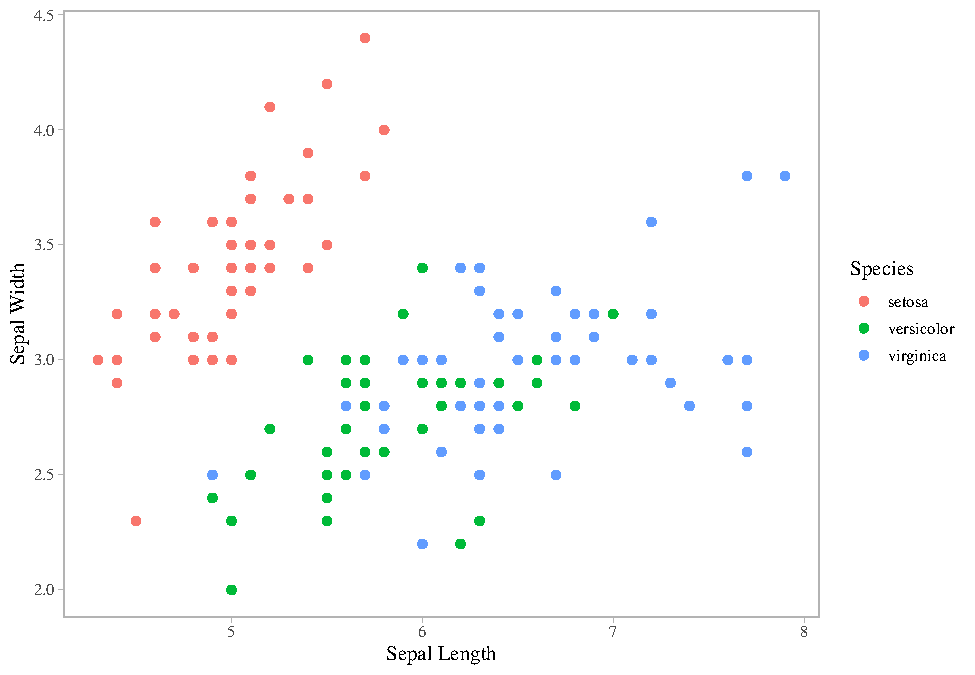
\includegraphics{best_practices_files/figure-latex/unnamed-chunk-1-1.pdf}

\hypertarget{rmarkdown}{%
\subsection{Rmarkdown}\label{rmarkdown}}

\emph{Note: This section is under development}

What is markdown?

\begin{itemize}
\item
  a very lightweight writing format originally created for conversion to
  HTML (a ``markup'' language - that is a pain to write)
\item
  it is plain text (no proprietary software - looking at you MS Word) so
  can be tracked via git\\
\item
  what can it be converted to?\\
  pdf, word, html
\item
  How does that work? via a program called Pandoc (a ``universal''
  document converter) - don't worry it is included with RStudio.
\end{itemize}

When to use it

-Whenever you want to rapidly communicate annotated code (informal
report) -Initial report writing\\
-To keep notes for yourself

Structure\\
* YAML - `YAML Ain't Markup Language' a human (and computer) readable
data format. This is the ``frontmatter'' of your report that tells
markdown what type of output you would like to have.\\
* there are a slew of options
\url{http://rmarkdown.rstudio.com/html_document_format.html} - I've
generally found that keeping it rather basic e.g.,

\begin{Shaded}
\begin{Highlighting}[]
\SpecialCharTok{{-}{-}{-}}
\NormalTok{title}\SpecialCharTok{:} \StringTok{\textquotesingle{}This is a title\textquotesingle{}}
\NormalTok{author}\SpecialCharTok{:} \StringTok{\textquotesingle{}Me\textquotesingle{}}
\NormalTok{date}\SpecialCharTok{:} \StringTok{"2017\_06\_10"}
\NormalTok{output}\SpecialCharTok{:}\NormalTok{pdf\_document}
\NormalTok{fontsize}\SpecialCharTok{:}\NormalTok{ 11pt}
\NormalTok{csl}\SpecialCharTok{:}\NormalTok{ canjfas.csl}
\NormalTok{bibliography}\SpecialCharTok{:}\NormalTok{ bibby.bib}
\SpecialCharTok{{-}{-}{-}}
\end{Highlighting}
\end{Shaded}

This has a title, author and date that will be at the head of the
document. I've told it to generate a pdf and have included a
bibliography (.bibtex format) for references and am using the Canadian
Journal or Fisheries and Aquatic Sciences .csl (citation style language)
that format the references. Here is a good site for downloading .csl
styles \url{https://github.com/citation-style-language/styles}

\begin{Shaded}
\begin{Highlighting}[]
\FunctionTok{sessionInfo}\NormalTok{(}\FunctionTok{c}\NormalTok{(}\StringTok{"ggplot2"}\NormalTok{, }\StringTok{"FNGr"}\NormalTok{))}
\end{Highlighting}
\end{Shaded}

\begin{verbatim}
## R version 4.1.2 (2021-11-01)
## Platform: x86_64-w64-mingw32/x64 (64-bit)
## Running under: Windows 10 x64 (build 19044)
## 
## Matrix products: default
## 
## locale:
## [1] LC_COLLATE=English_United States.1252 
## [2] LC_CTYPE=English_United States.1252   
## [3] LC_MONETARY=English_United States.1252
## [4] LC_NUMERIC=C                          
## [5] LC_TIME=English_United States.1252    
## 
## attached base packages:
## character(0)
## 
## other attached packages:
## [1] ggplot2_3.3.6   fngr_0.0.0.9000
## 
## loaded via a namespace (and not attached):
##  [1] httr_1.4.3        pkgload_1.2.4     tidyr_1.2.0       jsonlite_1.8.0   
##  [5] modelr_0.1.8      brio_1.1.3        assertthat_0.2.1  highr_0.9        
##  [9] grDevices_4.1.2   cellranger_1.1.0  yaml_2.2.2        remotes_2.4.2    
## [13] sessioninfo_1.2.2 Rttf2pt1_1.3.10   pillar_1.7.0      backports_1.4.1  
## [17] glue_1.6.1        base_4.1.2        extrafontdb_1.0   digest_0.6.29    
## [21] rvest_1.0.2       colorspace_2.0-3  htmltools_0.5.2   pkgconfig_2.0.3  
## [25] devtools_2.4.3    broom_0.8.0       haven_2.5.0       fngr_0.0.0.9000  
## [29] purrr_0.3.4       scales_1.2.0      processx_3.5.2    tzdb_0.3.0       
## [33] tibble_3.1.6      farver_2.1.0      generics_0.1.2    datasets_4.1.2   
## [37] usethis_2.1.6     ellipsis_0.3.2    cachem_1.0.6      withr_2.5.0      
## [41] tidyverse_1.3.1   cli_3.1.1         magrittr_2.0.2    crayon_1.5.1     
## [45] readxl_1.4.0      memoise_2.0.1     evaluate_0.15     ps_1.6.0         
## [49] methods_4.1.2     fs_1.5.2          fansi_1.0.3       forcats_0.5.1    
## [53] xml2_1.3.3        utils_4.1.2       pkgbuild_1.3.1    tools_4.1.2      
## [57] prettyunits_1.1.1 hms_1.1.1         lifecycle_1.0.1   stringr_1.4.0    
## [61] munsell_0.5.0     reprex_2.0.1      stats_4.1.2       callr_3.7.0      
## [65] compiler_4.1.2    rlang_1.0.2       grid_4.1.2        rstudioapi_0.13  
## [69] graphics_4.1.2    labeling_0.4.2    rmarkdown_2.14    testthat_3.1.2   
## [73] gtable_0.3.0      DBI_1.1.2         curl_4.3.2        R6_2.5.1         
## [77] lubridate_1.8.0   knitr_1.39        dplyr_1.0.8       fastmap_1.1.0    
## [81] extrafont_0.18    utf8_1.2.2        rprojroot_2.0.3   readr_2.1.2      
## [85] desc_1.4.1        stringi_1.7.6     vctrs_0.4.0       dbplyr_2.1.1     
## [89] tidyselect_1.1.2  xfun_0.30
\end{verbatim}

\end{document}
